\documentclass[12pt]{article}
\usepackage{amsmath}
\usepackage{array}
\usepackage{cancel}
\usepackage[thinc]{esdiff}
% \usepackage{gensymb}
\usepackage{geometry}
\usepackage{graphicx}
\usepackage{pgfplots}
\usepackage{siunitx}
\usepackage{wrapfig}
\usepackage{xcolor}

\pgfplotsset{compat=1.18}

\begin{document}
\section*{Problem 70}
\begin{wrapfigure}{r}{0.25\textwidth}
    \vspace{-30pt}
    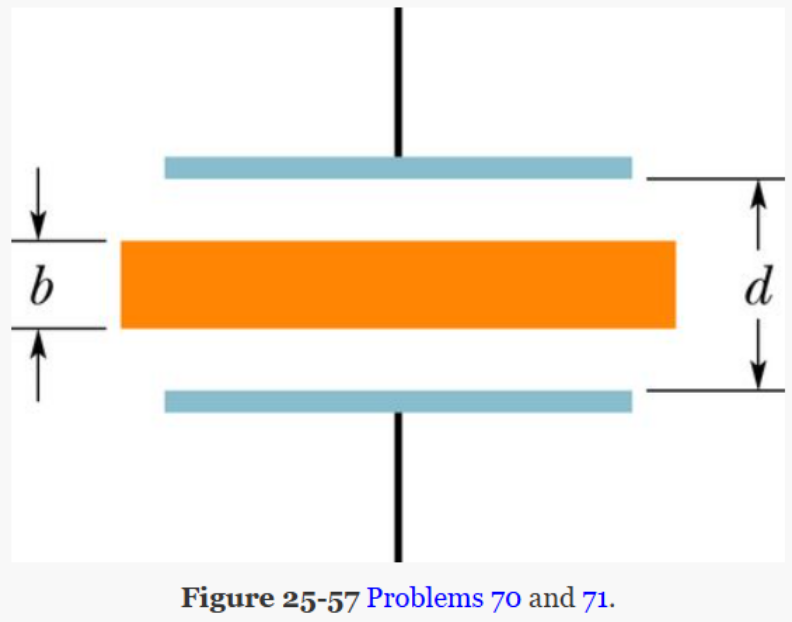
\includegraphics[width=0.25\textwidth]{image.png} 
    % \label{fig:wrapfig}
\end{wrapfigure}
A slab of copper of thickness $b = 2.00\unit{\milli\meter}$ is thrust into a parallel plate capacitor of plate area $A = 2.40 \unit{\centi\meter^2}$ and the plate separation is $d = 5.00 \unit{\milli\meter}$, as shown in the figure; the slab is exactly halfway between the plates. 
(a) What is the capacitance after the slab is introduced? 
(b) If a charge $q = 3.40\unit{\micro\coulomb}$ is maintained on the plates, what is the ratio of the energy stored before to that after the slab is introduced? 
(c) How much work is done on the slab as it is inserted? 
(d) Is the slab sucked in or meant to be pushed in?

\subsection*{Solution (a)}
The capacitance of the capacitor before the slab is inserted is calculatable.
\begin{align*}
    C   &=  \frac{\varepsilon_0 A}{d}
        =   \frac{8.85 \times 10^{-12} * 2.4 \times 10^{-4}}{5 \times 10^{-3}}
        =   4.248 \times 10^{-13} \unit{\farad}
\end{align*}

We can treat the capacitor as an equivalent to three different capacitors. 
The first and last capacitor would have the same areas, distances ($(5 - 2) / 2 = 1.5 \unit{\milli\meter}$ in this case), and capacitances.
Since copper is a conductor, its dielectric constant is essentially zero, so we can assume it to turn any fraction it is in the denominator to zero (and numerator to infinity),
\begin{align*}
    C_{eq}^{-1} &=  \frac{1}{C_1} + \frac{1}{C_2} + \frac{1}{C_3}
        =   \frac{2}{C_1} + \frac{1}{C_2}
        =   2*\frac{1.5 \times 10^{-3}}{\varepsilon_0 A} + \frac{2.0 \times 10^{-3}}{\kappa \varepsilon_0 A}
        =   \frac{3 \times 10^{-3}}{\varepsilon_0 A}\\
        &=  \frac{3 \times 10^{-3}}{8.85 \times 10^{-12} * 2.4 \times 10^{-4}}
        =   \frac{3}{21.24 \times 10^{-13}}\\
    C_{eq}  &=  \boxed{7.08 \times 10^{-13} \unit{\farad}}
\end{align*}

\subsection*{Solution (b)}
We have an equation for this.
\begin{align*}
    U   &=  \frac{q^2}{2C}
        % =   \frac{(3.4 \times 10^{-6} \unit{\coulomb})^2}{2 * 4.248 \times 10^{-13}}
\end{align*}

However, the only thing that changes between these is the capacitance.
We can set up a ratio for before and after.
\begin{align*}
    \frac{U_{before}}{U_{after}}    &=  \frac{q^2}{2C_{before}} * \frac{2C_{after}}{q^2}
        =   \frac{C_{after}}{C_{before}}
        =   \frac{7.08}{4.248}
        =   \boxed{1.67}
\end{align*}

\subsection*{Solution (c)}
Work done is equal to the change in potential energy.
\begin{align*}
    W   &=  U_f - U_i
        =   \frac{q^2}{2C_{after}} - \frac{q^2}{2C_{before}}
        =   \frac{(3.40 \times 10^{-6})^2}{2*4.248} - \frac{(3.40 \times 10^{-6})^2}{2*7.08}\\
        &=  
        =   \boxed{5.44 \times 10^{-13} \unit{\joule}}
\end{align*}

\subsection*{Solution (d)}
Since the work done is positive, it would follow that the slab would be exerted force on from outside. 
The answer is that it would be \underline{pushed in}.
\section*{Problem 71}
Repeat problem 70, assuming that a potential difference $V = 85.0 \unit{\volt}$, rather than the charge, is held constant.

\subsection*{Solution (a)}
Capacitance is not dependent on electric potential difference unless it's exploding. 
Thus, we have the same answer.
\boxed{7.08 \times 10^{-13} \unit{\farad}}

\subsection*{Solution (b)}
We have an equation for this. 
\begin{equation*}
    U = \frac{1}{2}CV^2
\end{equation*}

We just have to set up a ratio again.
The only thing that changes is still the capacitance.
\begin{align*}
    \frac{U_{before}}{U_{after}}    &=  \frac{\frac{1}{2}C_{before}V}{\frac{1}{2}C_{after}V}
        =   \frac{C_{before}}{C_{after}}
        =   \frac{4.248}{7.08}
        =   \boxed{0.6}
\end{align*}

\subsection*{Solution (c)}
Same as in Problem 70.
\begin{align*}
    W   &=  U_f - U_i
        =   \frac{1}{2}V^2(C_{after} - C_{before})
        =   \frac{85^2}{2}(4.248 - 7.08)
        =   \boxed{-10230.6 \unit{\joule}}
\end{align*}

\subsection*{Solution (d)}
Same as in Problem 70. 
Since the work done is negative, it would follow that the slab would not be exerted force on from outside. 
The answer is that it would be \underline{sucked in}.
\section*{Problem 45}
A certain parallel plate capacitor is filled with a dielectric for which $\kappa = 5.5$. 
The area of each plate is $0.034 \unit{\meter^2}$, and the plates are separated by $2.0 \unit{\milli\meter}$. 
The capacitor will fail if the electric field between the plates exceeds $200\unit{\kilo\newton/\coulomb}$. 
What is the maximum energy that can be stored in the capacitor?

\subsection*{Solution}
We have our equation for the capacitance of a parallel place capacitor ($C = \frac{\kappa\varepsilon_0A}{d}$).
For a parallel plate capacitor, the electrical field can generally be considered constant, so we can apply an algebraic equation ($V = Ed$).
Given the capacitance and electric potential difference, we can calculate the electrical potential energy of a charged capacitor ($U = \frac{1}{2}CV^2$).
\begin{align*}
    C   &=  \frac{\kappa\varepsilon_0A}{d}\\
    V   &=  Ed\\
    U   &=  \frac{1}{2}CV^2
        =   \frac{1}{2}*\frac{\kappa\varepsilon_0 A}{d} E^2 d^2
        =   \frac{1}{2}*\kappa\varepsilon_0 A E^2 d\\
        &=  \frac{1}{2} * 5.5 * (8.85 \times 10^{-12}) * 0.034 * \left(2 \times 10^5\right)^2 * 2 \times 10^{-3}\\
        &=  \boxed{6.6198 \times 10^{-5} \unit{\joule}}
\end{align*}

\end{document}